\hypertarget{dairy-queen}{%
\section{Dairy Queen}\label{dairy-queen}}

\begin{figure}[!ht]
  \begin{adjustwidth}{-\oddsidemargin-1in}{-\rightmargin}
    \centering
    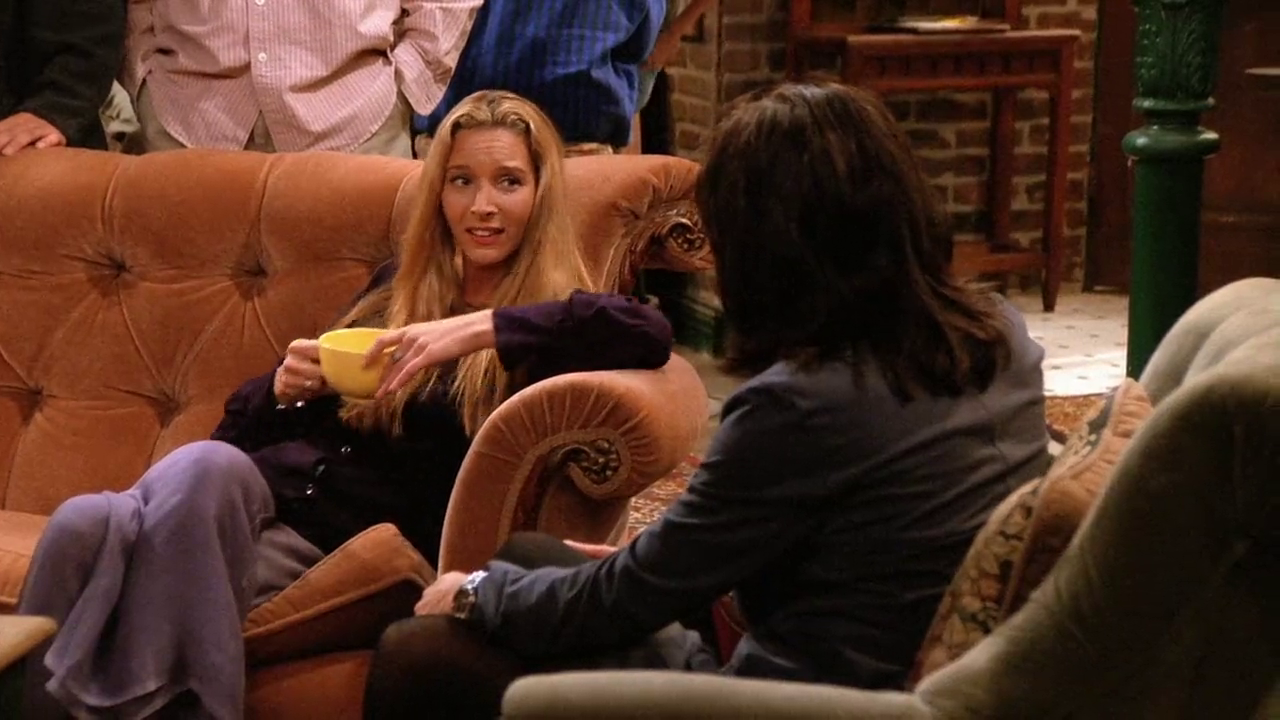
\includegraphics[trim={0 7cm 0 2cm,}, clip, width=\paperwidth]{./S01/img/4/dairy-queen.png}
    \caption{Dairy Queen\label{fig:dairy-queen}}
  \end{adjustwidth}
\end{figure}

\begin{tcolorbox}[enhanced,center upper,
    drop fuzzy shadow southeast, boxrule=0.3pt,
    lower separated=false,
    colframe=black!30!dialogoBorder,colback=white]
\begin{minipage}[c]{0.14\linewidth}
  \raisebox{\dimexpr-\height+\ht\strutbox\relax}{
    
\includegraphics[width=1.5cm]{./assets/img/phoebe.png}
  }
   & \centering \scriptsize{Phoebe}
\end{minipage}
\hspace{.1mm}
\begin{minipage}[c]{0.8\linewidth}
  \textbf{- There was a cave-in in one of the mines, and eight people were killed.}\\
  - Uma mina desabou e oito pessoas morreram.
\end{minipage}

\medskip
\begin{minipage}[c]{0.14\linewidth}
  \raisebox{\dimexpr-\height+\ht\strutbox\relax}{
    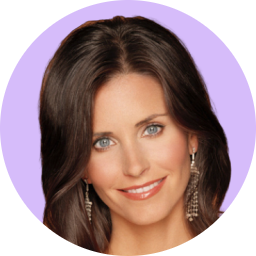
\includegraphics[width=1.5cm]{./assets/img/monica.png}
  }
   & \centering \scriptsize{Monica}
\end{minipage}
\hspace{.1mm}
\begin{minipage}[c]{0.8\linewidth}
  \textbf{- Wow, you worked in a mine?}\\
  - Trabalhou em uma mina?
\end{minipage}

\medskip
\begin{minipage}[c]{0.14\linewidth}
  \raisebox{\dimexpr-\height+\ht\strutbox\relax}{
    
\includegraphics[width=1.5cm]{./assets/img/phoebe.png}
  }
   & \centering \scriptsize{Phoebe}
\end{minipage}
\hspace{.1mm}
\begin{minipage}[c]{0.8\linewidth}
  \textbf{- No, I worked at a Dairy Queen. Why?}\\
  - Não, em um Dairy Queen. Por quê?
\end{minipage}
\end{tcolorbox}

Enquanto discutem sobre empregos e salários, Phoebe menciona um de seus
empregos em uma mina. Monica fica abismada com o fato e quer saber se
aquilo era verdade. Phoebe, sarcasticamente, responde que não, na
verdade era um \emph{Dairy Queen}.

\emph{Dairy Queen} (1940) é uma famosa rede de sorveterias e
restaurantes de \emph{fast-food}.

\hypertarget{referuxeancias}{%
\subsection{Referências}\label{referuxeancias}}

\begin{itemize}
\tightlist
\item
  \sloppy Site oficial. \url{https://dairyqueen.com/}
\item
  \sloppy Fórum WordReference (Inglês). \url{https://forum.wordreference.com/threads/dairy-queen-mine.1442748/}
\end{itemize}

\hypertarget{rachel-has-left-the-building}{%
\section{Rachel has left the
building}\label{rachel-has-left-the-building}}

\begin{figure}[!ht]
  \begin{adjustwidth}{-\oddsidemargin-1in}{-\rightmargin}
    \centering
    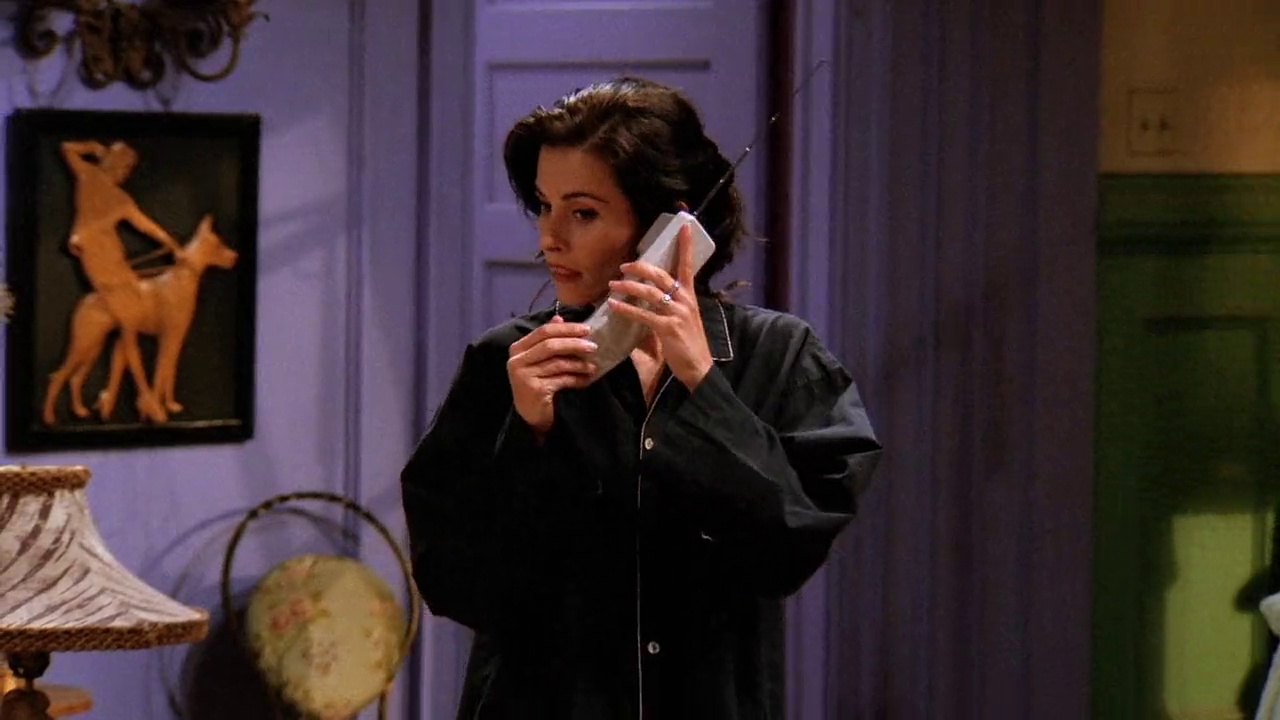
\includegraphics[trim={0 6cm 0 2cm,}, clip, width=\paperwidth]{./S01/img/4/rachel-has-left-the-building.png}
    \caption{Rachel has left the building\label{fig:rachel-has-left-the-building}}
  \end{adjustwidth}
\end{figure}

\begin{tcolorbox}[enhanced,center upper,
    drop fuzzy shadow southeast, boxrule=0.3pt,
    lower separated=false,
    colframe=black!30!dialogoBorder,colback=white]
\begin{minipage}[c]{0.14\linewidth}
  \raisebox{\dimexpr-\height+\ht\strutbox\relax}{
    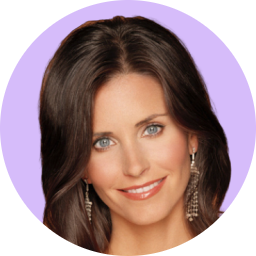
\includegraphics[width=1.5cm]{./assets/img/monica.png}
  }
   & \centering \scriptsize{Monica}
\end{minipage}
\hspace{.1mm}
\begin{minipage}[c]{0.8\linewidth}
  \textbf{- Rachel has left the building.}\\
  - Rachel deixou o edifício.
\end{minipage}
\end{tcolorbox}

Após atender a um telefonema da operadora de cartão perguntando sobre a
Rachel, Monica diz a frase \emph{Rachel has left the building}. Isto é
uma paráfrase de \emph{Elvis has left the building}. Era uma frase usada
para dispersar o público que ficava a espera do bis ao final do show do
Rei do \emph{Rock and Roll Elvis Presley}.

\hypertarget{referuxeancias-1}{%
\subsection{Referências}\label{referuxeancias-1}}

\begin{itemize}
\tightlist
\item
  \sloppy Fandom Wiki. \url{https://friends.fandom.com/wiki/The_One_With_George_Stephanopoulos}
\item
  \sloppy Wikipédia. \url{https://en.wikipedia.org/wiki/Elvis_has_left_the_building}
\end{itemize}

\hypertarget{jack-and-the-beanstalk}{%
\section{Jack and the Beanstalk}\label{jack-and-the-beanstalk}}

\begin{figure}[!ht]
  \begin{adjustwidth}{-\oddsidemargin-1in}{-\rightmargin}
    \centering
    
\includegraphics[trim={0 6cm 0 2cm,}, clip, width=\paperwidth]{./S01/img/4/jack-and-the-beanstalk.png}
    \caption{Jack and the Beanstalk\label{fig:jack-and-the-beanstalk}}
  \end{adjustwidth}
\end{figure}

\begin{tcolorbox}[enhanced,center upper,
    drop fuzzy shadow southeast, boxrule=0.3pt,
    lower separated=false,
    colframe=black!30!dialogoBorder,colback=white]
\begin{minipage}[c]{0.14\linewidth}
  \raisebox{\dimexpr-\height+\ht\strutbox\relax}{
    
\includegraphics[width=1.5cm]{./assets/img/phoebe.png}
  }
   & \centering \scriptsize{Phoebe}
\end{minipage}
\hspace{.1mm}
\begin{minipage}[c]{0.8\linewidth}
  \textbf{- You are just like Jack.}\\
  - Você é igual ao João.
\end{minipage}

\medskip
\begin{minipage}[c]{0.14\linewidth}
  \raisebox{\dimexpr-\height+\ht\strutbox\relax}{
    
\includegraphics[width=1.5cm]{./assets/img/rachel.png}
  }
   & \centering \scriptsize{Rachel}
\end{minipage}
\hspace{.1mm}
\begin{minipage}[c]{0.8\linewidth}
  \textbf{- Jack from downstairs?}\\
  - João, do andar de baixo?
\end{minipage}

\medskip
\begin{minipage}[c]{0.14\linewidth}
  \raisebox{\dimexpr-\height+\ht\strutbox\relax}{
    
\includegraphics[width=1.5cm]{./assets/img/phoebe.png}
  }
   & \centering \scriptsize{Phoebe}
\end{minipage}
\hspace{.1mm}
\begin{minipage}[c]{0.8\linewidth}
  \textbf{- No, Jack and the Beanstalk.}\\
  - Não, João e o Pé de Feijão.
\end{minipage}
\end{tcolorbox}

\emph{Jack and the Beanstalk} (1807), conhecido no Brasil como
\emph{João e o Pé de Feijão}, é um conto de fadas de origem inglesa. A
Phoebe conta bem o enredo da história na cena. É uma história bastante
conhecida e referenciada diversas vezes, como em \emph{O Pica-pau},
\emph{Mickey Mouse}, entre outros.

\hypertarget{referuxeancias-2}{%
\subsection{Referências}\label{referuxeancias-2}}

\begin{itemize}
\tightlist
\item
  \sloppy Página da Universidade de Pittsburgh (Inglês). \url{https://www.pitt.edu/~dash/type0328jack.html}
\end{itemize}

\hypertarget{george-stephanopoulos}{%
\section{George Stephanopoulos}\label{george-stephanopoulos}}

\begin{figure}[!ht]
  \begin{adjustwidth}{-\oddsidemargin-1in}{-\rightmargin}
    \centering
    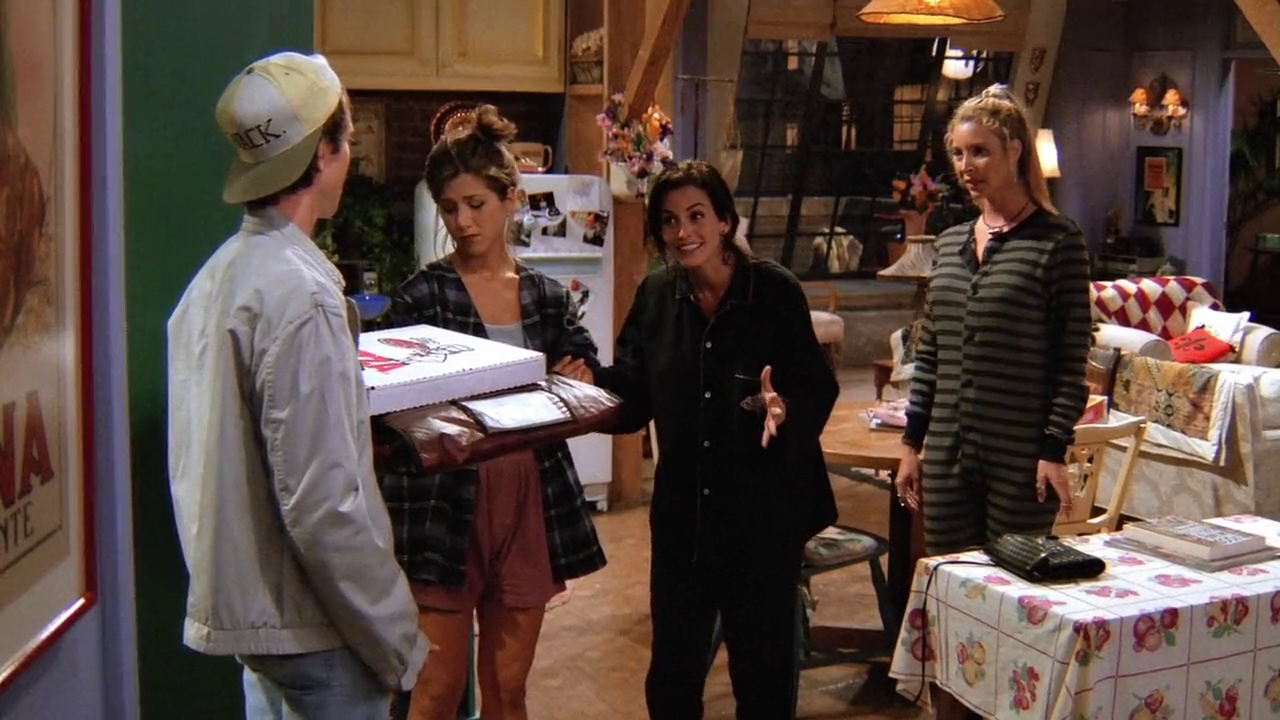
\includegraphics[trim={0 7cm 0 2cm,}, clip, width=\paperwidth]{./S01/img/4/george-stephanopoulos.png}
    \caption{George Stephanopoulos\label{fig:george-stephanopoulos}}
  \end{adjustwidth}
\end{figure}

\begin{tcolorbox}[enhanced,center upper,
    drop fuzzy shadow southeast, boxrule=0.3pt,
    lower separated=false,
    colframe=black!30!dialogoBorder,colback=white]
\begin{minipage}[c]{0.14\linewidth}
  \raisebox{\dimexpr-\height+\ht\strutbox\relax}{
    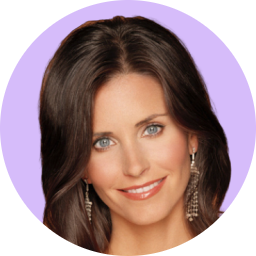
\includegraphics[width=1.5cm]{./assets/img/monica.png}
  }
   & \centering \scriptsize{Monica}
\end{minipage}
\hspace{.1mm}
\begin{minipage}[c]{0.8\linewidth}
  \textbf{- Did you say G. Stephanopoulos?}\\
  - Calma, você falou G. Stephanopoulos?
\end{minipage}
\end{tcolorbox}

\emph{George Stephanopoulos} (1961-) realmente existe e na época dessa
temporada era diretor de comunicações da campanha presidencial de Bill
Clinton. Atualmente é, entre outras coisas, âncora do telejornal
\emph{Good Morning America}.

Essa passagem de sua vida virou o documentário \emph{The War Room}
(1993).

\begin{figure}
  \centering
  \begin{tikzpicture}
    \node [inner sep=0pt] at (0,0) {
      
\includegraphics[width=0.8\textwidth,keepaspectratio]{./S01/img/4/george-stephanopoulos-war-room.jpg}
    };
    \draw [white, rounded corners=\ClipSep, line width=\ClipSep]
    (current bounding box.north west) --
    (current bounding box.north east) --
    (current bounding box.south east) --
    (current bounding box.south west) -- cycle
    ;
    \end{tikzpicture}
    \caption{George Stephanopoulos - The War Room\label{fig:george-stephanopoulos-the-war-room}}
\end{figure}

\hypertarget{referuxeancias-3}{%
\subsection{Referências}\label{referuxeancias-3}}

\begin{itemize}
\tightlist
\item
  \sloppy Twitter. \url{https://twitter.com/gstephanopoulos}
\item
  \sloppy IMDB. \url{https://www.imdb.com/name/nm0826888/?ref_=tt_ov_st_sm}
\item
  \sloppy IMDB Documentário. \url{https://www.imdb.com/title/tt0108515/}
\end{itemize}

\hypertarget{george-snuffleupagus}{%
\section{George ``Snuffleupagus''}\label{george-snuffleupagus}}

\begin{figure}[!ht]
  \begin{adjustwidth}{-\oddsidemargin-1in}{-\rightmargin}
    \centering
    
\includegraphics[trim={0 6cm 0 1cm,}, clip, width=\paperwidth]{./S01/img/4/george-snuffleupagus.png}
    \caption{George ``Snuffleupagus''\label{fig:george-snuffleupagus}}
  \end{adjustwidth}
\end{figure}

\begin{tcolorbox}[enhanced,center upper,
    drop fuzzy shadow southeast, boxrule=0.3pt,
    lower separated=false,
    colframe=black!30!dialogoBorder,colback=white]
\begin{minipage}[c]{0.14\linewidth}
  \raisebox{\dimexpr-\height+\ht\strutbox\relax}{
    
\includegraphics[width=1.5cm]{./assets/img/rachel.png}
  }
   & \centering \scriptsize{Rachel}
\end{minipage}
\hspace{.1mm}
\begin{minipage}[c]{0.8\linewidth}
  \textbf{- Who's George Snuffleupagus?}\\
  - Quem é George Snuffleupagus?
\end{minipage}

\medskip
\begin{minipage}[c]{0.14\linewidth}
  \raisebox{\dimexpr-\height+\ht\strutbox\relax}{
    
\includegraphics[width=1.5cm]{./assets/img/phoebe.png}
  }
   & \centering \scriptsize{Phoebe}
\end{minipage}
\hspace{.1mm}
\begin{minipage}[c]{0.8\linewidth}
  \textbf{- That's Big Bird's friend.}\\
  - Amigo do Garibaldo.
\end{minipage}
\end{tcolorbox}

Rachel confunde o sobrenome de George e o chama de \emph{Snuffleupagus}.
Ele é realmente amigo de \emph{Big Bird} e, ambos, fazem parte do
programa de televisão educacional \emph{Sesame Street} (1969), conhecido
no Brasil como \emph{Vila Sésamo}. Em nossa versão, \emph{Snuffleupagus}
era \emph{Funga-Funga} (à direita) e \emph{Big Bird} era
\emph{Garibaldo} (à esquerda).

\begin{figure}
  \centering
  \begin{tikzpicture}
    \node [inner sep=0pt] at (0,0) {
      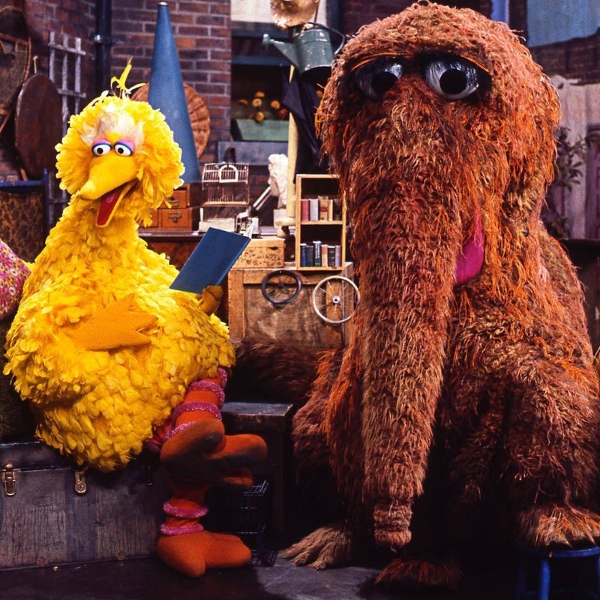
\includegraphics[width=0.5\textwidth,keepaspectratio]{./S01/img/4/snuffleupagus-big-bird.jpg}
    };
    \draw [white, rounded corners=\ClipSep, line width=\ClipSep]
    (current bounding box.north west) --
    (current bounding box.north east) --
    (current bounding box.south east) --
    (current bounding box.south west) -- cycle
    ;
    \end{tikzpicture}
    \caption{Snuffleupagus e Big Bird\label{fig:snuffleupagus-e-big-bird}}
\end{figure}

\hypertarget{referuxeancias-4}{%
\subsection{Referências}\label{referuxeancias-4}}

\begin{itemize}
\tightlist
\item
  \sloppy Fandom Wiki - Mr. Snuffleupagus. \url{https://muppet.fandom.com/wiki/Mr._Snuffleupagus}
\item
  \sloppy Fandom Wiki - Big Bird. \url{https://muppet.fandom.com/wiki/Big_Bird}
\item
  \sloppy Site oficial - Sesame Street. \url{https://www.sesamestreet.org/}
\end{itemize}

\hypertarget{silence-of-the-lambs}{%
\section{Silence of the Lambs}\label{silence-of-the-lambs}}

\begin{figure}[!ht]
  \begin{adjustwidth}{-\oddsidemargin-1in}{-\rightmargin}
    \centering
    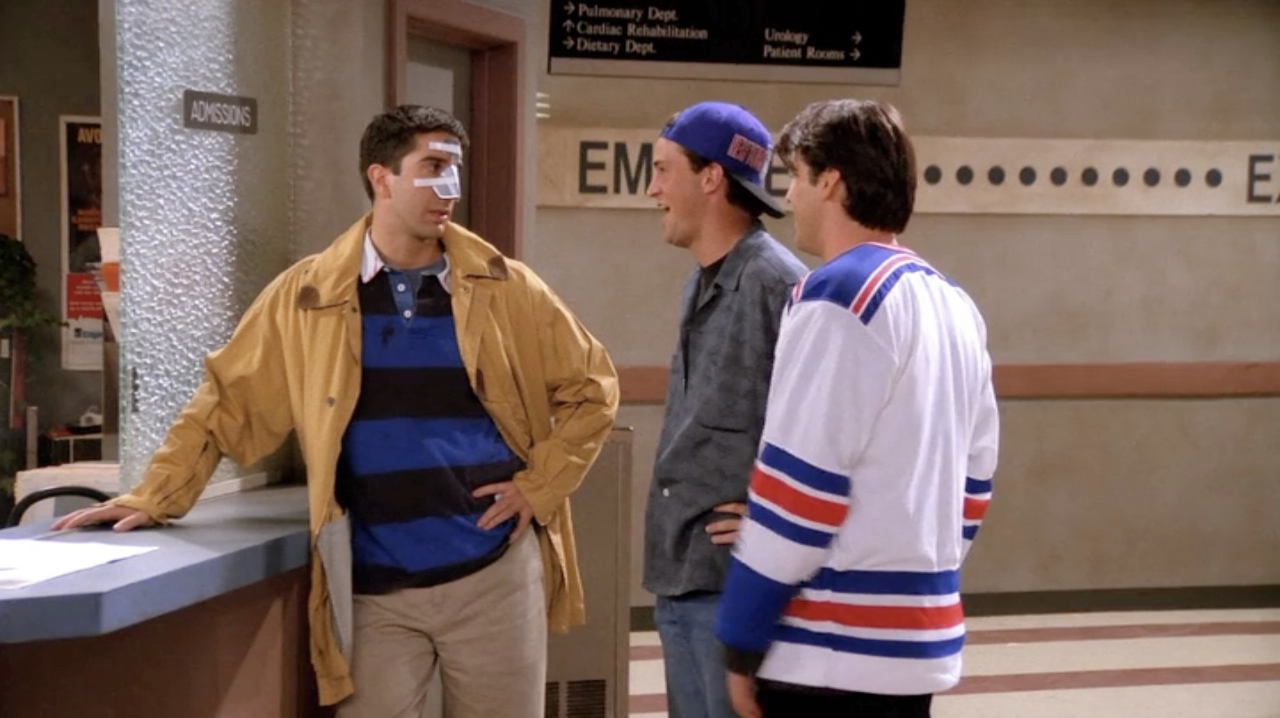
\includegraphics[trim={0 7cm 0 2cm,}, clip, width=\paperwidth]{./S01/img/4/silence-of-the-lambs.png}
    \caption{Silence of the Lambs\label{fig:silence-of-the-lambs}}
  \end{adjustwidth}
\end{figure}

\begin{tcolorbox}[enhanced,center upper,
    drop fuzzy shadow southeast, boxrule=0.3pt,
    lower separated=false,
    colframe=black!30!dialogoBorder,colback=white]
\begin{minipage}[c]{0.14\linewidth}
  \raisebox{\dimexpr-\height+\ht\strutbox\relax}{
    
\includegraphics[width=1.5cm]{./assets/img/chandler.png}
  }
   & \centering \scriptsize{Chandler}
\end{minipage}
\hspace{.1mm}
\begin{minipage}[c]{0.8\linewidth}
  \textbf{- Oh, I thought you were great in Silence of the Lambs.}\\
  - Você estava ótimo em Silêncio dos Inocentes.
\end{minipage}
\end{tcolorbox}

\emph{Silence of the Lambs} (1991) é um filme norte-americano de
suspense, drama e terror, estrelado por \emph{Jodie Foster} e
\emph{Anthony Hopkins}. A comparação feita por Chandler se refere ao
modo como o \emph{Dr.~Hannibal Lecter}, interpretado por \emph{Hopkins},
era transportado quando precisava sair da cadeia. No Brasil o filme
ficou conhecido como \emph{Silêncio dos Inocentes}.

\begin{figure}
  \centering
  \begin{tikzpicture}
    \node [inner sep=0pt] at (0,0) {
      
\includegraphics[width=0.8\textwidth,keepaspectratio]{./S01/img/4/hannibal-lecter.jpg}
    };
    \draw [white, rounded corners=\ClipSep, line width=\ClipSep]
    (current bounding box.north west) --
    (current bounding box.north east) --
    (current bounding box.south east) --
    (current bounding box.south west) -- cycle
    ;
    \end{tikzpicture}
    \caption{Hannibal Lecter\label{fig:hannibal-lecter}}
\end{figure}

\hypertarget{referuxeancias-5}{%
\subsection{Referências}\label{referuxeancias-5}}

\begin{itemize}
\tightlist
\item
  \sloppy IMDB. \url{https://www.imdb.com/title/tt0102926/}
\item
  \sloppy Wikipédia. \url{https://pt.wikipedia.org/wiki/O_Sil%C3%AAncio_dos_Inocentes}
\end{itemize}
